% Hello emacs, this is -*- latex -*-
\typeout{ ====================================================================}
\typeout{ This is file implement.tex, created at 02-Nov-2006 }
\typeout{ Maintained by Andre Anjos <Andre.dos.Anjos@cern.ch> }
\typeout{ ====================================================================}

\chapter{Desempenho computacional do sistema de discriminação}
\label{chap:implement}

O algoritmo apresentado nesta seção deve respeitar as normas de operação do
Segundo Nível de Filtragem do experimento. Neste nível de filtragem, espera-se
que o tempo médio de processamento para cada evento, incluindo acesso aos
dados no sistema de leitura, seja de 10 milissegundos. No entanto, espera-se
que o sistema opere rejeitando eventos ordinários o mais rápido possível, de
tal forma que, estatisticamente, a maior parte do tempo despendida nos
processadores do LVL2 seja dedicada a eventos interessantes.

Levando-se em consideração que o tempo de acesso aos dados no sistema de
leitura está na ordem de 1~ms, como descrito no Capítulo~\ref{chap:trigger},
deseja-se minimizar o tempo de processamento despendido no algoritmo. Desta
forma, medidas de desempenho são normalmente executadas nos candidatos a
algoritmos ao sistema de filtragem, de modo a determinar seu tempo de execução
e possíveis pontos a serem otimizados. O correto balanço entre a rejeição
prematura de um evento e o número de requisições de dados deve ser feita, de
forma a otimizar tanto seu acesso quanto seu processamento. Isto ocorre pois
existe uma dependência direta entre os dois parâmetros a serem considerados: o
número de requisições de dados interrompe o processamento para se aguardar a
informação requisitada. Quanto mais informação, mais processamento deverá ser
realizado para o tratamento dos dados. Deseja-se, desta forma, minimizar o
acesso a dados e maximizar a capacidade discriminativa do sistema.

Nossa referência, o algoritmo do T2Calo, foi completamente descrita na
Seção~\ref{sec:lvl2-detect-electron}. Neste algoritmo, inicia-se o
processamento detetando-se o pico na segunda camada e.m., seguindo-se do
cálculo da variável $\rcore$. A variável $\eratio$ é calculada em seguida,
utilizando-se dos dados da primeira camada e.m.. De posse dos valores parciais
de energia nestas duas camadas, os dados do pré-irradiador e da terceira
camada e.m. são utilizados para definir o valor da variável $\etem$. Na última
parte do processamento define-se o valor da variável $\ethad$, acessando-se os
dados da parte hadrônica. A Tabela~\ref{tab:t2calo-performance} contém as mais
recentes medidas realizadas na avaliação do desempenho do T2Calo
\cite{denis-presentation}. Os valores nesta tabela representam o tempo médio
de processamento, em milissegundos, para cada uma das fases. Estes tempos
também desconsideram a execução do algoritmo de hipótese EGammaHypo. Assume-se
no entanto, que seja desprezível, dado sua simplicidade.

\begin{table}
\caption{Tempo de processamento médio (em milissegundos) das diversas fases do
algoritmo T2Calo em uma máquina com processadores Intel Xeon de 2,4 GHz e 1~Gb
de memória RAM.}
\label{tab:t2calo-performance}
\begin{center}
\begin{tabular}{|l|r|r|r|} \hline
\textbf{Fase} & \textbf{Prep. Dados} & 
\textbf{Algoritmo} & \textbf{Tot. parcial}\\ \hline
$\rcore$ & 0,45 & 0,49 & 0,94 \\ 
$\eratio$ & 0,48 & 0,57 & 1,05 \\ 
$\etem$ & 0,56 & 0,17 & 0,73 \\ 
$\ethad$ & 0,59 & 0,33 & 0,92 \\ \hline
\textbf{Total} & \textbf{2,08} & \textbf{1,56} & \textbf{3,64} \\ \hline
\end{tabular}
\end{center}
\end{table}

Tomando-se por base que um sistema baseado no anelamento e deteção neural terá
que acessar os mesmos dados das mesmas fontes que aquelas acessadas pelo
T2Calo, em uma primeira aproximação e sem se considerar quaisquer processos de
otimização, a primeira parte do tempo (Calibração e Localização na tabela)
deve ser tomada como constante. A segunda parte, no entanto, é completamente
dependente do algoritmo e devemos compará-la ao tempo de execução do
\eng{NeuralRinger}.

A complexidade de execução do método baseado no anelador e deteção neural é
variável de acordo com dois parâmetros principais:

\begin{enumerate}
\item Com o número de anéis que se deseja extrair: neste caso, quanto mais
anéis deseja-se extrair dos dados, maior o tempo de execução que será
necessário para cumprir o processo de anelamento. Ademais, com o aumento do
número de anéis aumenta-se igualmente o tamanho da entrada do discriminador
neural e, portanto, o número de operações aritméticas para esta última fase do
processamento;
\item O número de neurônios escondidos na rede neural também influenciará o
tempo de execução do discriminador.
\end{enumerate}

Para determinar a viabilidade em termos de desempenho, para o algoritmo proposto
por este trabalho, executou-se a aplicação \texttt{ringer-run} em um conjunto
de máquinas de referência ao experimento ATLAS. A
Tabela~\ref{tab:machine-comparison} resume as características destas
máquinas. A primeira das máquinas listadas está sendo utilizada em uma
avaliação de arquiteturas para o sistema de filtragem e aquisição de dados do
ATLAS, conhecido como \textit{pré-série} \cite{gokhan-chep06}. Esta é a
máquina de referência máxima para estudos de desempenho no ATLAS. A segunda
máquina de teste é um modelo com dois núcleos (\eng{dual-core}). A arquitetura
desta máquina está sendo considerada como opção às máquinas atualmente
empregadas nas pré-séries, sendo este modelo de processador o mais recente
disponibilizado pelo fabricante. A terceira e última máquina faz parte de um
conjunto de máquinas dedicado a estudos do sistema de filtragem. Embora possua
uma arquitetura mais antiga, ainda é usada como referência em muitos
trabalhos, sendo este o caso das medidas do T2Calo apresentadas acima.

\begin{table}
\caption{Configurações das máquinas utilizadas para o teste de desempenho do
\eng{NeuralRinger}.}
\label{tab:machine-comparison}
\begin{center}
\begin{tabular}{|l|l|r|r|} \hline
Processador & \eng{Clock} & \eng{Cache} de L2 & Memória RAM \\ \hline
AMD Opteron (250) & 2,4~GHz & 1~Mb & 4~Gb \\
AMD Opteron (275) & 2,2~GHz & 1~Mb & 4~Gb \\
Intel Xeon & 2,4~GHz & 512~kb & 1~Gb \\ \hline
\end{tabular}
\end{center}
\end{table}

Estas máquinas contêm uma instalação completamente funcional do sistema
operacional atualmente empregado no CERN, o SLC3 \cite{cern-linux}. Embora
alguns dos processadores possam operar em 64-bits (assim como o
\eng{NeuralRinger}), estas máquinas são operadas em modo de compatibilidade
para 32-bits, já que grande parte do \eng{software} do ATLAS ainda não opera
corretamente em 64-bits.

Um conjunto idêntico, composto de três diferentes testes foram executados em
cada uma das máquinas, utilizando todos os dados disponíveis (cerca de 22.600
elétrons e 7500 jatos) para este estudo. Para estes testes, utilizou-se o
programa \texttt{ringer-run}, que executa as fases de anelamento e
discriminação em seqüência, como aconteceria num sistema \eng{online}.  Os
testes realizados em uma mesma máquina diferem entre si somente pela
configuração de anelamento e da rede neural que discriminará os dados após a
extração dos anéis. As combinações utilizadas equivalem àquelas dos testes
mostrados no Capítulo~\ref{chap:neural}, para o sistema com 100 anéis, um
sistema podado com 34 anéis e o último, utilizando apenas 14 anéis mais
relevantes. Durante os testes, observou-se a quantidade de memória RAM
disponível na máquina de tal forma que o carregamento dos dados não ativasse o
mecanismo de troca de disco (do inglês, \eng{swap}), já que isso faria com que
a aplicação tivesse um desempenho abaixo do esperado para o experimento.

As Figuras~\ref{fig:timings-histo-full}, \ref{fig:timings-histo-cut1} e
\ref{fig:timings-histo-cut2} contém os resultados dos 3 testes com 100, 34 e
14 anéis, respectivamente, nas três arquiteturas. Das três arquiteturas
escolhidas, a máquina da pré-série parece ser a mais rápida, apresentando um
tempo de processamento de apenas $445$ microssegundos para o mais complexo dos
testes, utilizando 100 anéis. Em seguida, o sistema baseado no processador
Opteron-275, cerca de 8\% mais lento para o mesmo teste. A máquina de testes
do sistema de filtragem é a mais lenta de todas as plataformas, apresentando
um tempo médio de processamento de $542$ microssegundos para cada RoI. O
desvio-padrão está na faixa dos 10\%, indicando uniformidade nos resultados.

\begin{figure}
\begin{center}
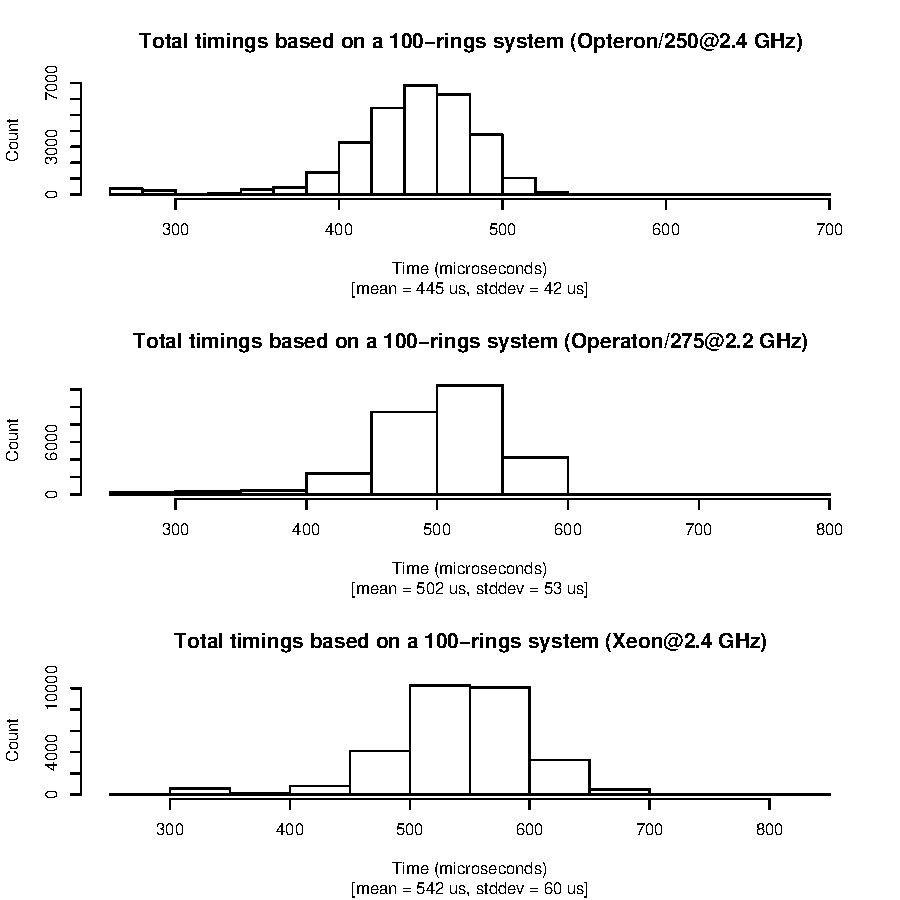
\includegraphics[scale=0.98]{ringer-mlp/compare-test-full-rings}
\end{center}
\caption{Tempos totais de execução do \eng{NeuralRinger} em três plataformas
distintas, utilizando 100 anéis.}
\label{fig:timings-histo-full}
\end{figure}

\begin{figure}
\begin{center}
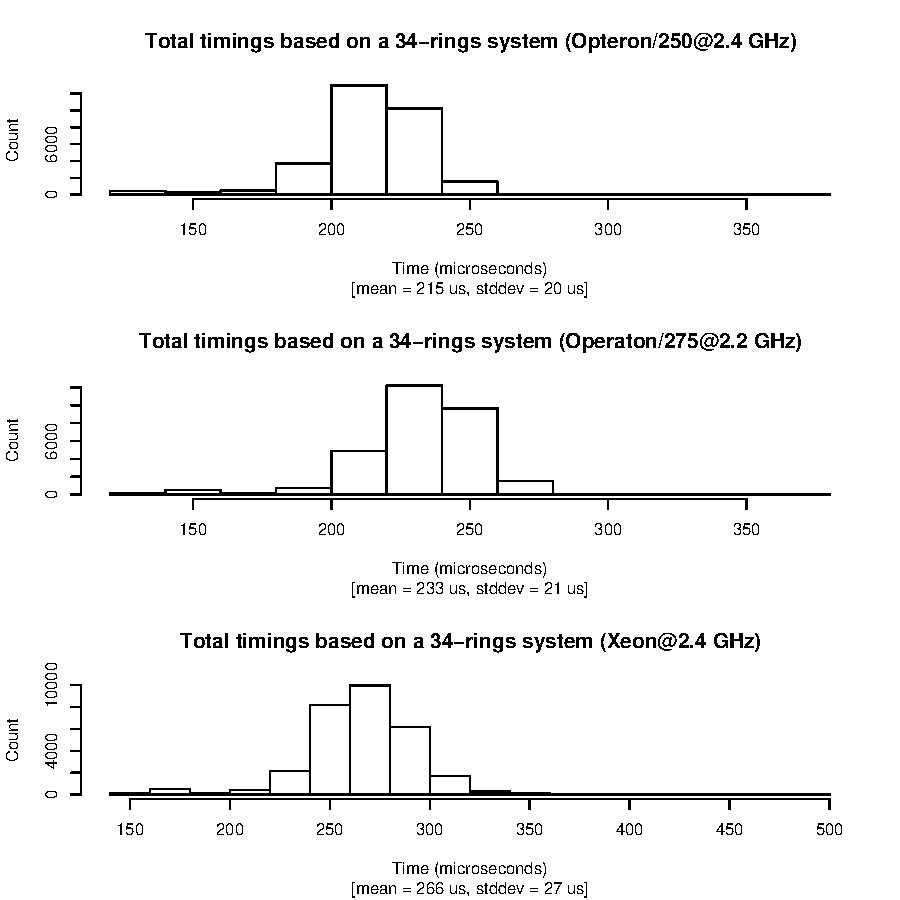
\includegraphics[scale=0.98]{ringer-mlp/compare-test-cut1-rings}
\end{center}
\caption{Tempos totais de executava do \eng{NeuralRinger} em três plataformas
distintas, utilizando 34 anéis.}
\label{fig:timings-histo-cut1}
\end{figure}

\begin{figure}
\begin{center}
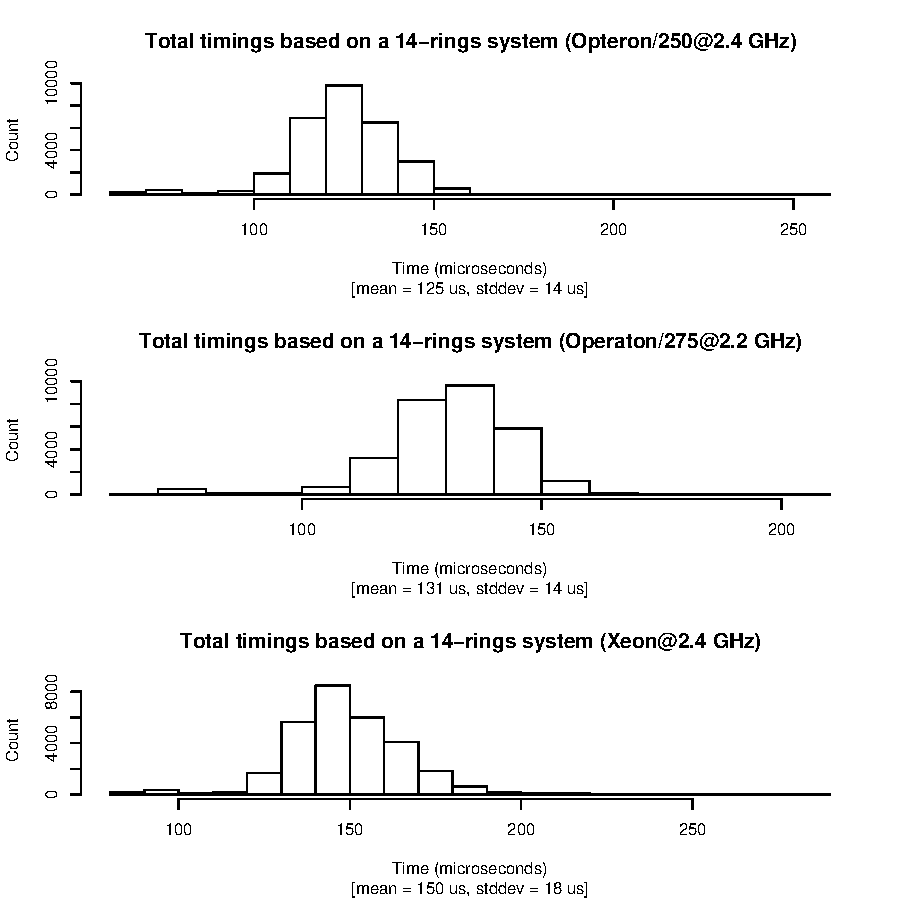
\includegraphics[scale=0.98]{ringer-mlp/compare-test-cut2-rings}
\end{center}
\caption{Tempos totais de execração do \eng{NeuralRinger} em três plataformas
distintas, utilizando apenas 14 anéis.}
\label{fig:timings-histo-cut2}
\end{figure}

Nos testes seguintes, a relação entre o desempenho das máquinas se
mantém. Para o teste com 34 anéis o tempo de processamento médio na máquina
mais rápida é de $215$ microssegundos, tendo caído aproximadamente a metade do
valor para os 100 anéis. Para o teste com apenas 14 dos 100 anéis originais, o
tempo médio de processamento é de apenas $125$ microssegundos para a máquina
mais veloz, representando quase um-quarto do tempo de processamento para o
sistema de anelamento completo.

Ao compararmos os resultados dos testes com 100 anéis ao tempo de referência
do T2Calo (1,56~ms) para a mesma plataforma, observa-se que o sistema proposto
executa em apenas um-terço do tempo requerido para o T2Calo nesta
arquitetura. Esta análise não leva em conta o acesso aos dados e sua
calibração e localização dentro das bibliotecas de infraestrutura do LVL2. No
entanto, por inspeção à Tabela~\ref{tab:t2calo-performance}, nota-se que cerca
de 57\% do tempo total do processamento de uma RoI, isto é, aproximadamente
2,1~ms é devido a esta parte dos dados. Desta forma, conclui-se que o sistema
proposto pelo anelador está dentro das especificações de desempenho para o
sistema de filtragem do ATLAS.

A Figura~\ref{fig:p1-full-histos} mostra os histogramas individuais para cada
uma das fases de processamento, para o teste usando 100 anéis rodando na
máquina mais rápida (Opteron/250, 2,4~GHz). Desta figura conclui-se que, no
caso de tempos de processamento menores se tornarem imperativos, uma
implementação dedicada do processo de anelamento (originalmente implementado
na biblioteca \texttt{rbuild}) poderá ser realizada de forma que o tempo total
de deste algoritmo seja otimizado. Junto à discriminação neural as duas fases
representam mais de 90\% do tempo de processamento total. Otimizações na fase
de procura do pico de deposição energética na segunda camada e.m. ou na fase
de normalização dos anéis teriam quase ou nenhum impacto considerando-se a
arquitetura atual do \eng{NeuralRinger}.

\begin{figure}
\begin{center}
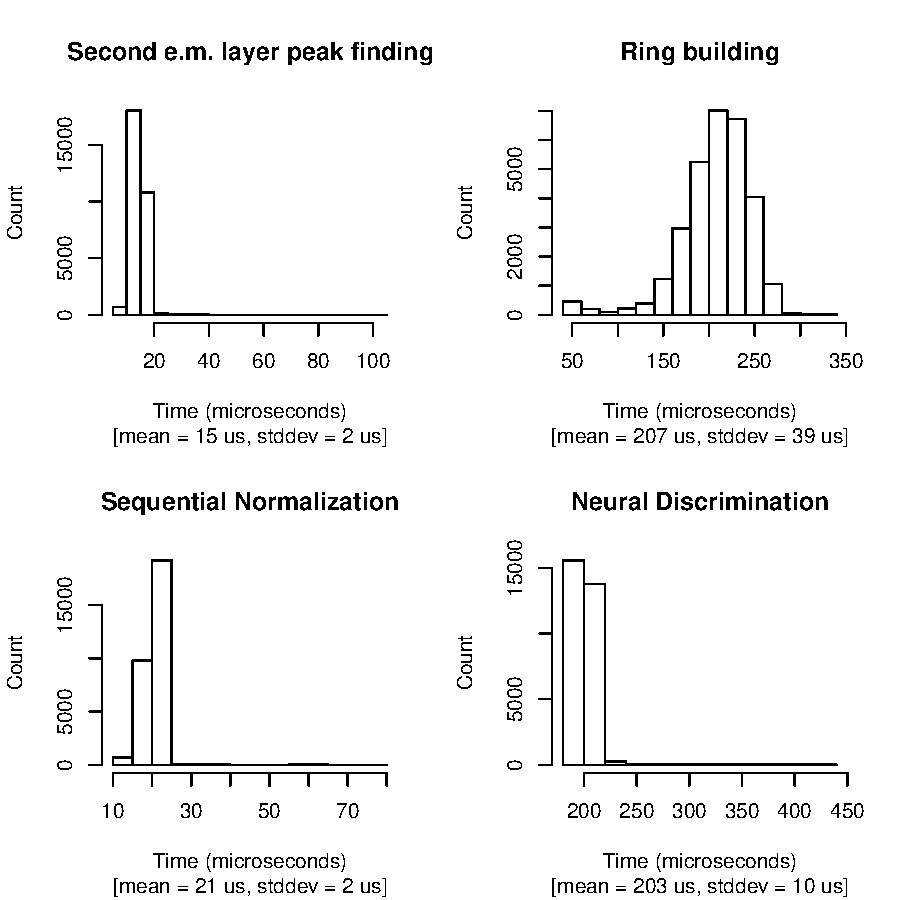
\includegraphics[scale=0.98]{ringer-mlp/full-histos-opteron-250}
\end{center}
\caption{Tempos individuais para cada fase de execução do \eng{NeuralRinger},
levando-se em consideração a extração e discriminação baseada em 100 anéis. O
teste foi executado na plataforma Opteron/250 (pré-serie).}
\label{fig:p1-full-histos}
\end{figure}

\section{Migração para o Sistema de Filtragem do ATLAS}

Algoritmos candidatos ao Sistema de Filtragem do ATLAS não devem somente ter
bom desempenho, mas também atender todos os critérios e restrições de operação
neste árduo ambiente. Em específico, o ambiente de trabalho deste sub-sistema
do experimento contém as primitivas de acesso aos dados e calibração assim
como a lógica que coordena o processo de filtragem. Mesmo embebido dentro
desta, muitas vezes pesada, arquitetura, o algoritmo deve manter um desempenho
compatível seu propósito: filtragem ultra-veloz. Nesta seção abordamos a
arquitetura e implementação do sistema de anelamento e processamento neural
dentro do Sistema de Filtragem do experimento ATLAS e, sobretudo, ao ambiente
de desenvolvimento Athena \cite{athena:home-page, athena:devel-guide}, que
permite o transporte destas ferramentas entre os dois mundos do experimento:
filtragem e análise \eng{offline}.

O \eng{NeuralRinger} evoluiu ao longo de 2 anos de desenvolvimento de forma
que se tornasse facilmente integrável ao ambiente de funcionamento
\eng{online}, que é baseado no ambiente de desenvolvimento Athena. Uma vez
integrado, o \eng{NeuralRinger} poderá extrair anéis da RoI seguindo uma
determinada configuração de anelamento e aplicar um processo de decisão
baseado em uma rede neural pré-configurada. A implementação de um detetor
neural baseado na técnica de anelamento, neste contexto, deve seguir os
seguintes passos:

\begin{enumerate}
\item Encontrar os dados que serão utilizados para treino e teste do
discriminador neural. Rodar o programa \texttt{athena}, de forma a extrair
dados no formato nativo do \eng{NeuralRinger};
\item Projetar e treinar o sistema de anelamento e detetor neural no ambiente
do \eng{NeuralRinger}, totalmente desconectado do Sistema de Filtragem do
ATLAS;
\item Aplicar as configurações de anelamento e deteção neural no sistema
\eng{online}.
\end{enumerate}

Desta forma, é possível desacoplar o desenvolvimento de detetores ao uso do
ambiente Athena, o que é uma vantagem considerável: diminui-se o tempo de
desenvolvimento e permite-se que o usuário foque sua atenção ao problema da
classificação sem se importar com os detalhes, muitas vezes complexos, deste
ambiente. Os resultados da aplicação de um detetor específico, dentro e fora
do ambiente Athena devem ser idênticos.

\subsection{\eng{NeuralRinger} e o Athena}

Para que seja facilmente integrável dentro do ambiente Athena, o
\eng{NeuralRinger} segue a filosofia de funcionamento deste ambiente. Cada uma
das fases de processamento, i.e., a criação dos anéis de energia e a
classificação neural estão codificadas em bibliotecas individualizadas e podem
ser utilizadas tanto conjunta quanto separadamente. No ambiente
\eng{online}, a extração de características e deteção são normalmente
separadas de forma que possam ser desenvolvidas independentemente.

O processamento do evento dentro do sistema filtragem ocorre de forma
seqüencial, como explicado na Seção~\ref{sec:hlt}. Para cada objeto ou RoI
destacado pelo nível de filtragem antecedente, o componente do HLT conhecido
como \eng{Steering} (que poderia ser traduzido, neste contexto, como
Coordenador ou Agendador) irá definir o algoritmo que será chamado para
tratá-lo. O algoritmo poderá realizar um conjunto de operações no objeto em
questão, aumentando a quantidade de informações disponíveis para análise deste
ítem ou interrompendo o processamento.

Desta forma, é possível definir duas classes de algoritmos:

\begin{itemize}
\item \textbf{Extração}: Algoritmos que apenas adicionam informação a um
objeto no evento, através da extração de características nos dados do detetor;
\item \textbf{Hipótese}: Algoritmos que interrompem o processamento de um
objeto por considerarem-no como física ordinária que não deve ser registrada
em mídia permanente.
\end{itemize}

Sendo, o processo de hipótese, separado do processo de extração, é possível
desenvolver sistemas de decisão mais e mais complexos conforme se avance
dentro da análise do evento. A Figura~\ref{fig:simple-menu} exemplifica este
cenário para uma configuração fictícia para o \eng{Steering}. Este é um
exemplo que pode ser reproduzido no LVL2: um objeto tipo e.m. é encontrado no
resultado do LVL1 passado ao \eng{Steering}. Este objeto causa o agendamento
de um algoritmo que possa tratá-lo. A primeira fase do processamento é a
extração de características do objeto. Neste exemplo, a primeira extração de
característica considerada é a extração dos anéis. No passo seguinte a extração
é a hipótese (neural). Se o objeto atender às características de um elétron, o
\eng{Steering} irá agendar o passo seguinte. Caso, não, a hipótese de que o
objeto seja um objeto tipo e.m. é rejeitada e o processamento é parado,
causando a rejeição do evento pelo sistema de filtragem. Caso a hipótese seja
afirmativa, neste exemplo, tentar-se-á encontrar um traço relativo ao objeto
nos detetores de traço. Caso isto falhe, o objeto será rejeitado como indica a
figura. Se, finalmente, nenhuma das fases de processamento conseguir rejeitar
o objeto, ele será rotulado como um elétron, os valores extraídos das
características do objeto serão adicionados a este novo elemento e o evento
será aprovado.

\begin{figure}
\begin{center}
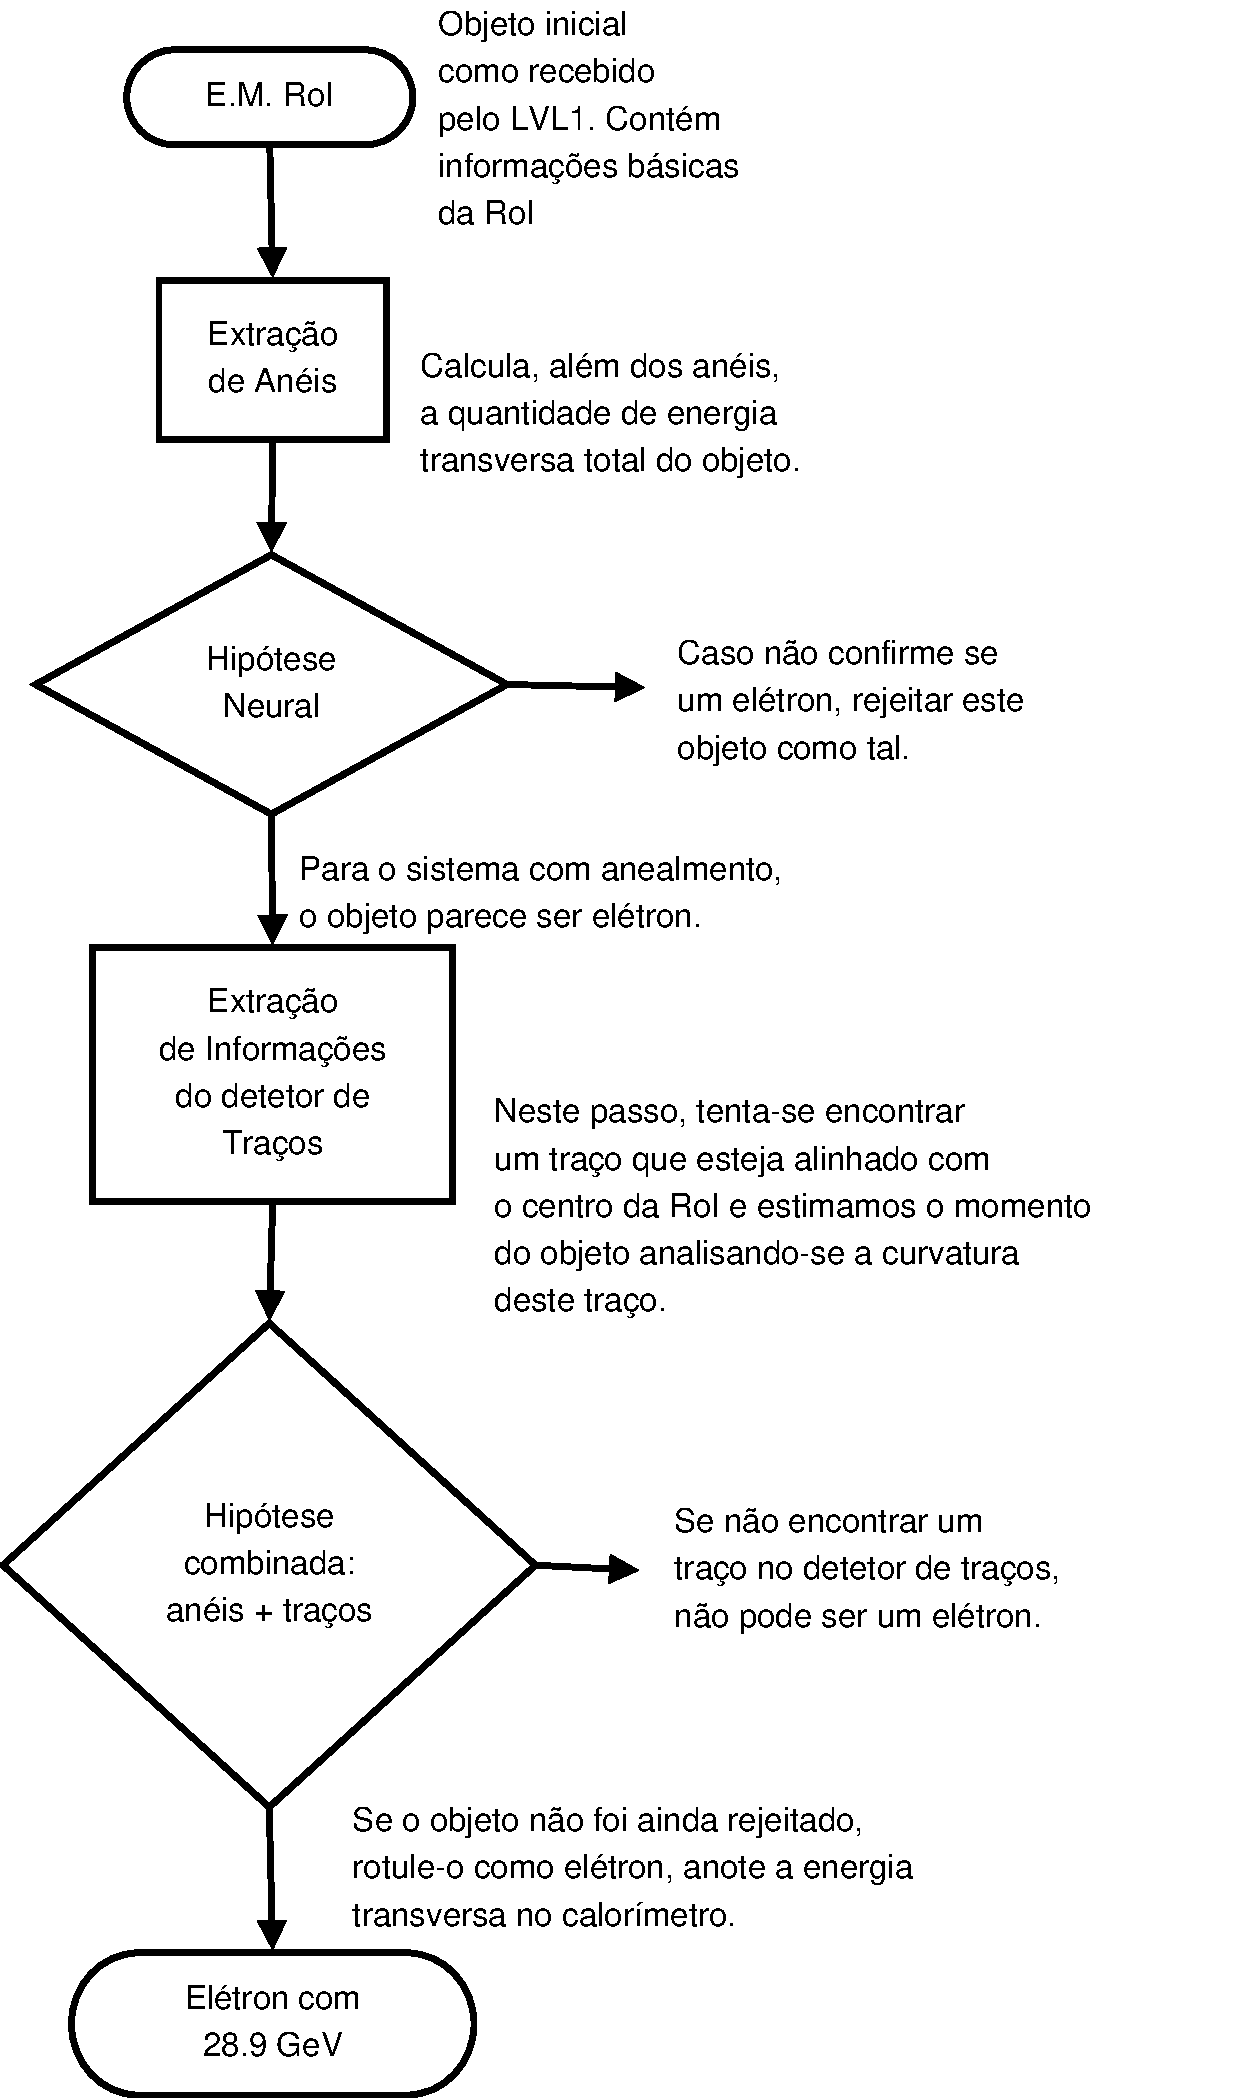
\includegraphics[scale=0.40]{simple-menu}
\end{center}
\caption{Exemplo de um cenário de seleção simples para o \eng{Steering}
operando no LVL2, baseado em uma RoI tipo E.M..}
\label{fig:simple-menu}
\end{figure}

Para atender à alta complexidade do experimento, muitas seqüências como a
descrita na Figura~\ref{fig:simple-menu} podem co-existir dentro do
\eng{Steering}. Cabe a este sistema de agendamento escolher a seqüência de
passos e combinações de objetos apropriadas para que se possa analisar o
evento adequadamente.

Para a integração do \eng{NeuralRinger} e observando-se a estrutura de
processamento \eng{online}, divide-se o anelamento e a decisão neural em dois
passos distintos, que podem ser executados independentemente. Para evitar a
dispersão de código, foram criados 3 pacotes:

\begin{itemize}
\item \textbf{TrigRingerTools}: Este pacote contém as bibliotecas 
originais do \eng{NeuralRinger} e é usado como base funcional dos outros
pacotes;
\item \textbf{TrigCaloRinger}: Este pacote implementa um algoritmo de 
extração de características. As características neste caso são os valores
energéticos dos anéis;
\item \textbf{TrigMultiVarHypo}: Este pacote implementa um algoritmo de
hipótese baseada em redes neurais. Nele encontra-se a implementação do
algoritmo de hipótese baseada em redes neurais. 
\end{itemize}

Com esta configuração é possível manter o conjunto de bibliotecas do
\eng{NeuralRinger} coeso em um único pacote (\texttt{TrigRingerTools}) e
apenas implementar um conjunto de algoritmos que usam a funcionalidade de base
deste pacote. Os algoritmos de extração de características e hipótese são
configuráveis em todos os aspectos da sua versão desacoplada e podem escrever
em disco os resultados parciais de suas operações para verificação externa ao
Athena.

Para determinar o correto funcionamento deste sistema, é necessário testar,
baseado na entrada, a saída de cada passo, para um conjunto de eventos. Para
tal, utilizou-se uma base de dados com eventos simulados tipo $Z \rightarrow
e^- + e^-$ que estava disponível no formato adequado. Uma configuração de
anelamento utilizando 100 anéis conforme descritos anteriormente, e uma rede
neural com 100 entradas, 8 neurônios escondidos e um neurônio na camada de
saída. Cerca de 850 RoI's foram selecionadas pela simulação do LVL1 indicando
objetos a serem averiguados no LVL2. Roda-se o sistema Athena, configurado
para utilizar os algoritmos de anelamento e deteção neural extraindo-se 3
tipos de dados:

\begin{enumerate}
\item O valores de energia e posicionamento das células utilizadas para o
cálculo dos anéis, num formato compatível com o padrão do \eng{NeuralRinger}; 
\item Uma base de dados de anéis já processados e normalizados, em formato
XML;
\item Uma base de dados com as saídas do processamento neural, também no
formato XML.
\end{enumerate}

Com base na versão desacoplada (\eng{standalone}, não integrada ao ambiente
Athena ou ao Sistema de Filtragem) do \eng{NeuralRinger}, executam-se os mesmos
processos:

\begin{enumerate}
\item Baseado nos valores originais das células provida pelo Athena, calculam-se
a soma de anéis; 
\item Baseado na saída dos anéis provida pelo Athena, calculam-se a saída da
rede neural.
\end{enumerate}

A Figura~\ref{fig:athena-vs-nr} mostra as diferenças, RoI a RoI, nos cenários
1 e 2 descritos anteriormente. Como é possível observar no primeiro histograma
desta figura, os resultados são idênticos com uma precisão melhor que $1
\times 10^{-7}$ no caso do Teste~1. Esta pequena diferença existe pois os
valores relativos às energias das células, escritos em disco para a análise
pelo \eng{NeuralRinger}, são truncados na décima casa decimal, por opção de
projeto. A propagação deste erro através da extração de anéis induz um erro
relativo aparentemente maior na saída deste processo.

\begin{figure}
\begin{center}
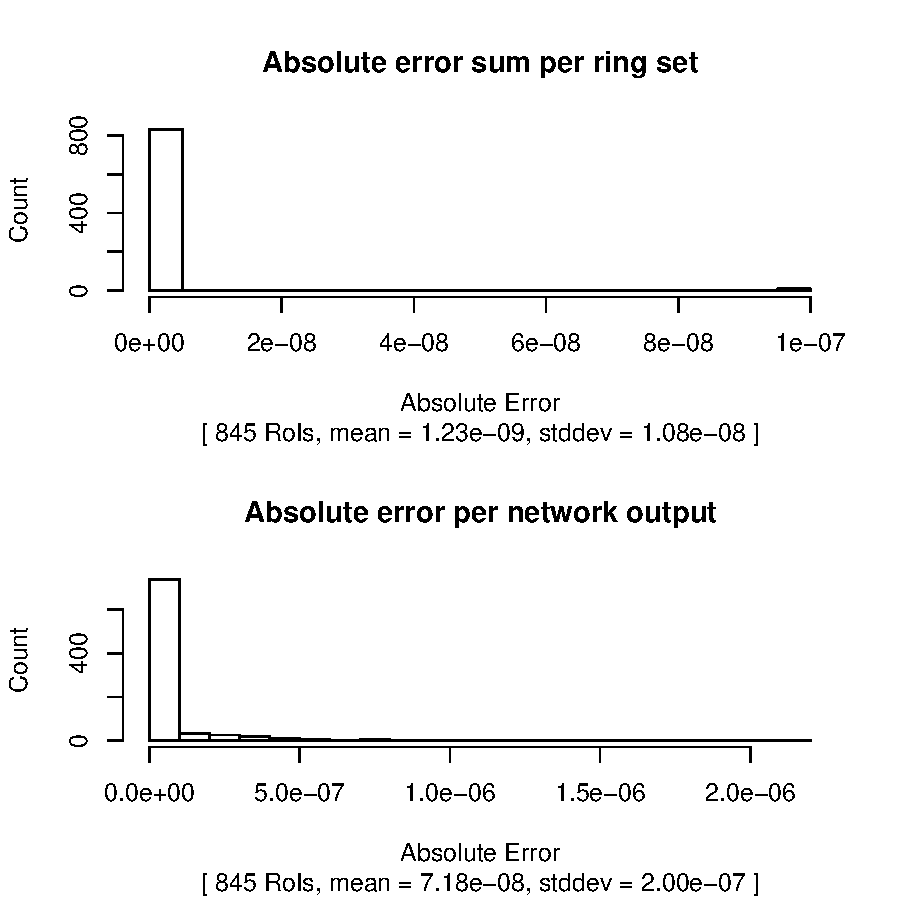
\includegraphics[scale=0.98]{athena-vs-nr-error}
\end{center}
\caption{Erros entre os processos de extração de características e hipótese
neural entre o Athena e o \eng{NeuralRinger} rodando em modo desacoplado.}
\label{fig:athena-vs-nr}
\end{figure}

Para o Teste~2, no histograma na parte inferior da
Figura~\ref{fig:athena-vs-nr}, o resultados são idênticos para uma precisão
melhor que $2 \times 10^{-6}$. Este erro existe pois os valores relativos às
energias dos anéis, escritos em disco para a análise pelo \eng{NeuralRinger},
são truncados a partir da sexta casa decimal.

Para completar a análise, roda-se o processo completo de extração e
classificação neural, baseando-se nos valores das células, comparando a saída
deste procedimento à saída provida pelo sistema neural acoplado ao ambiente
Athena. A Figura~\ref{fig:athena-vs-nr-full} mostra um gráfico de correlação
das saídas dos dois sistemas para as configurações de anelamento e rede neural
descritas anteriormente. Neste caso, onde não há escrita em disco entre os
dois passos do processamento, o erro observado é zero, entre os dois
sistemas. Estes resultados, portanto, indicam que a precisão de escrita é
suficiente para a reprodução desacoplada e que o sistema migrado funciona
adequadamente.
% Cabe-se notar que a rede neural utilizada para este teste não
%havia sido treinada para a deteção eficiente de dados com empilhamento, sendo
%esta a razão da distribuição tão homegênea da saída do detetor neural.

\begin{figure}
\begin{center}
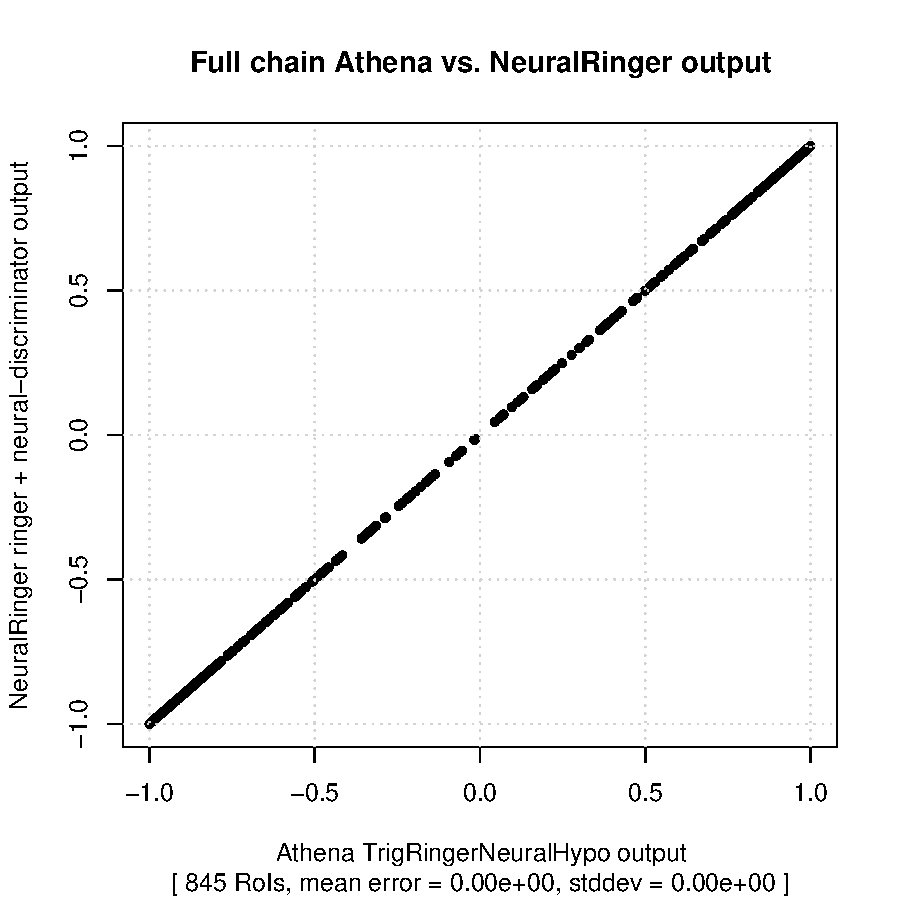
\includegraphics[scale=0.98]{athena-vs-nr-error-full-chain}
\end{center}
\caption{Gráfico de correlação entre a saída final do Athena e de uma versão do
\eng{NeuralRinger} rodando em modo desacoplado.}
\label{fig:athena-vs-nr-full}
\end{figure}

O segundo passo é a confirmação dos tempos de operação destacados ao longo do
texto. Neste caso, deseja-se averiguar se a migração não acarretou algum
impacto ao desempenho do sistema, uma vez que uma infraestrutura maior de
suporte à execução está sendo utilizada. Ademais, uma vez que se estará
realizando acesso remoto aos dados e calibração, processos que não são
executados no ambiente desacoplado, deseja-se estimar o impacto que estas
novas atividades causariam ao emprego do anelamento e discriminação neural no
Sistema de Filtragem. Por outro lado, obtém-se com este estudo um conjunto de
valores comparativos mais justos a outros métodos de deteção, tais como o
sistema proposto pelo T2Calo$+$EGammaHypo. Isto acontece pois estaremos
interfaceando com as diversas partes da infraestrutura de processamento do
Sistema de Filtragem da mesma forma. Por questões de praticidade ligadas à
disponibilidade dos dados e quantidade de memória disponível, escolhe-se a
máquina baseada no processador AMD Opteron $275$ utilizada anteriormente, para
realização dos testes.

\paragraph{Serviço de Temporização do Athena:} O serviço de temporização do
Athena (no pacote \eng{TrigTimeSvc}) utiliza a função \texttt{gettimeofday}
\cite{web:gcc-libc} para executar a operação de medida de tempo entre dois
pontos quaisquer dentro do código. A utilização de um relógio em tempo-real é
benéfica quando se deseja medir tempos de processamento com uma precisão menor
que 10~milissegundos (fornecida pela função \texttt{clock}). 

Um dos inconvenientes da função \texttt{gettimeofday} é que o valor obtido em
uma chamada é uma medida absoluta do tempo. Como um processo Unix está sujeito
a interrupções de sua execução (dado o compartilhamento da máquina por outros
processos e agentes), o tempo parado também será contado,
eventualmente. Ademais, máquinas modernas possuem normalmente mais de um
processador. É portanto provável que processos que estejam parados, neste
contexto, sejam mais rapidamente agendados. Desta forma, o tempo final
observado será uma mistura de tempos de execução reais, somados aos tempos de
parada e re-agendamento. Estes tempos não são normalmente significativos para
longos processos, mas podem facilmente afetar a percepção de processos mais
curtos. Para evitar que estes tipos de evento ocorram com freqüência durante a
medida de tempo, ajustou-se a prioridade de execução do processo Athena de
forma a minimizar o tempo que o processo estaria parado ou em transição de
processador.

A Figura~\ref{fig:timings-athena} mostra 7 histogramas correspondentes às
diversas fases do processamento do \eng{NeuralRinger} integrado ao ambiente
Athena. Na parte superior da figura, observa-se o tempo de acesso aos
dados. Este tempo de acesso é partilhado por todos os algoritmos de
calorimetria, e apresenta neste caso uma média de 2,2~milissegundos por
RoI. No ambiente Athena, este valor inclui o tempo de formatação dos dados no
padrão dos detetores do ATLAS. Os quatro histogramas que seguem representam
histogramas equivalentes aos da Figura~\ref{fig:p1-full-histos}, onde é
possível observar os tempos individuais de cada uma das fases do processo de
extração de características e classificação neural. Os dois histogramas no
final da figura mostram os tempos de processamento totais, por algoritmo.

\begin{figure}
\begin{center}
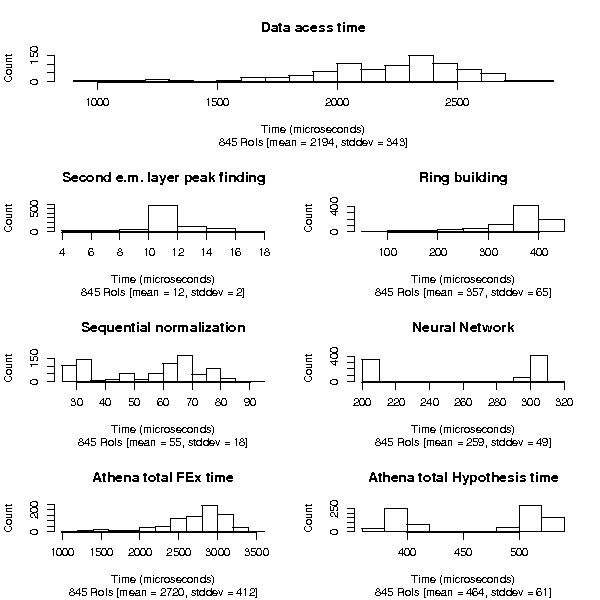
\includegraphics[scale=0.98]{timings-pcuwtr1}
\end{center}
\caption{Tempos de execução do \eng{NeuralRinger} funcionando de forma
integrada ao ambiente Athena.}
\label{fig:timings-athena}
\end{figure}

Removendo-se a contribuição do tempo de acesso aos dados, o processo de
extração leva em média $2720-2194=526$ microssegundos. O tempo médio de
classificação baseado em uma rede neural leva $259$ microssegundos. Desta
forma, o tempo total, comparável àquele da
Figura~\ref{fig:timings-histo-full}, é de $526+259=785$ microssegundos. Este
valor representa um acréscimo de cerca de 56\% do tempo total calculado
anteriormente. Uma parte do tempo adicional é gasto na criação de estruturas
de dados que sejam transportáveis entre os algoritmos, passo necessário no
ambiente Athena e que foi suprimido na execução desacoplada. Uma outra parte
advém da utilização da infraestrutura de acesso a dados e relatório de erros
disponível no ambiente Athena, que é mais lenta que no ambiente desacoplado.

O tempo total de processamento do algoritmo integrado é de cerca de
3,2~milissegundos. Comparando-se os tempos relativos de processamento para
diversas configurações de anéis e detetores neurais das
Figuras~\ref{fig:timings-histo-full}, \ref{fig:timings-histo-cut1} e
\ref{fig:timings-histo-cut2} observa-se uma relação aproximadamente constante
de cerca de 10 a 15\% de diferença entre as plataformas AMD Opteron-275 e
Intel Xeon, dependendo do número de anéis utilizados. Escalando o valor de
tempo observado considerando-se a diferença máxima de 15\%, chega-se a um
valor de $\approx 3,8$ milissegundos. Este valor é comparável ao tempo total
de processamento do T2Calo, na Tabela~\ref{tab:t2calo-performance}, de $3,64$
milissegundos. Portanto, com este exercício, demonstra-se a viabilidade deste
sistema de deteção para operação \eng{online}.

A Figura~\ref{fig:timings-eta-dep} ilustra a dependência dos tempos parciais
de processamento com a localização da região de interesse, por $\eta$. A
Figura~\ref{fig:timings-phi-dep} mostra a relação com a variável
$\phi$. Naturalmente, o processo é tendencioso com relação à variável $\eta$,
devido às variações da granularidade e independente da localização em $\phi$.

\begin{figure}
\begin{center}
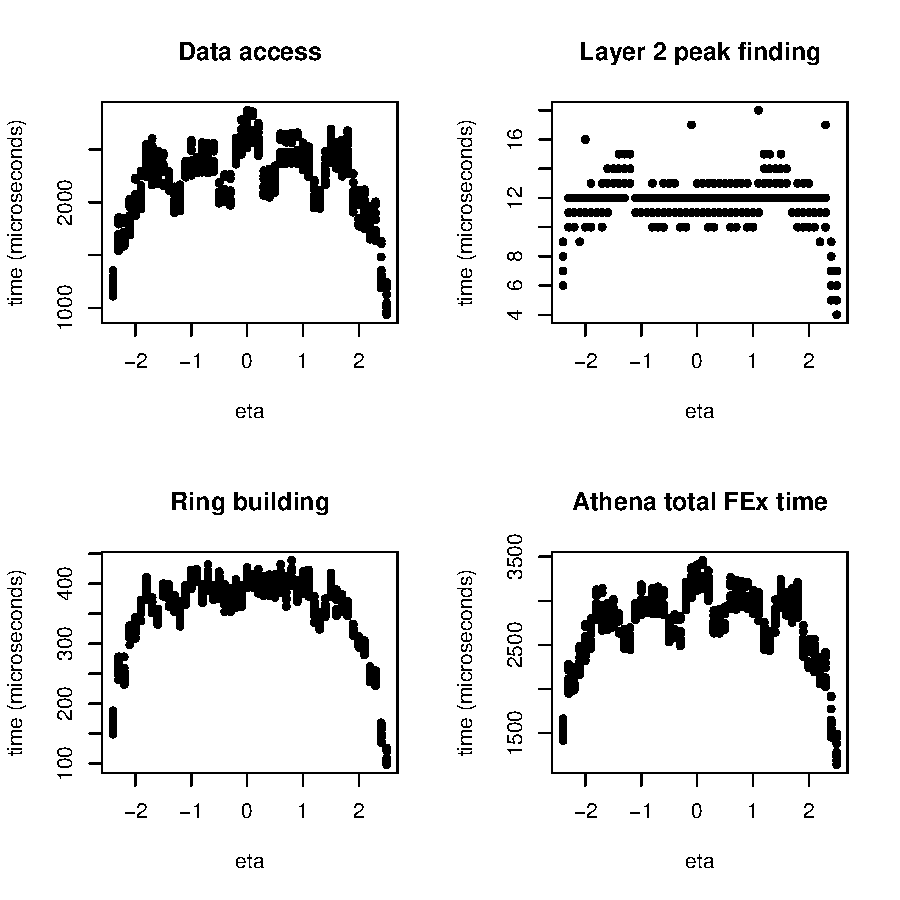
\includegraphics[scale=0.98]{timings-eta-dep}
\end{center}
\caption{Relação entre o posicionamento da RoI em $\eta$ e os tempos de
processamento do \eng{NeuralRinger} em diversas das fases da extração de
características no ambiente Athena.}
\label{fig:timings-eta-dep}
\end{figure}

\begin{figure}
\begin{center}
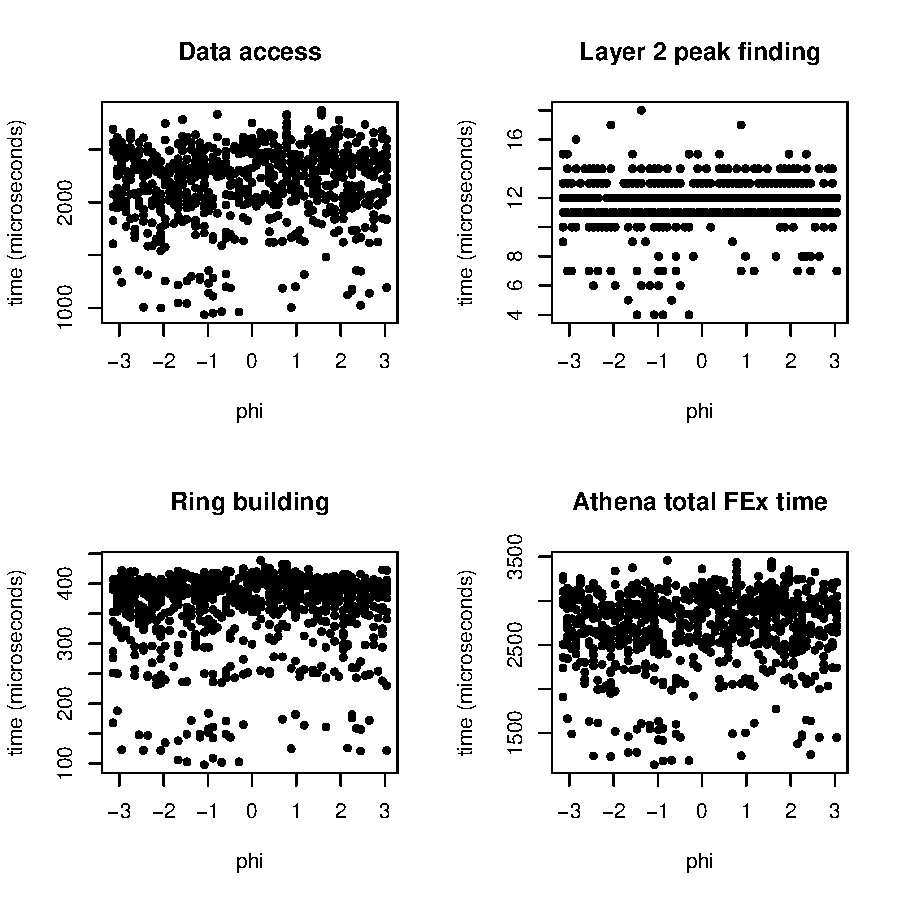
\includegraphics[scale=0.98]{timings-phi-dep}
\end{center}
\caption{Relação entre o posicionamento da RoI em $\phi$ e os tempos de
processamento do \eng{NeuralRinger} em diversas das fases da extração de
características no ambiente Athena.}
\label{fig:timings-phi-dep}
\end{figure}

\subsection{\eng{NeuralRinger} e o sistema de aquisição}

O último passo da integração é a demonstração da viabilidade do sistema de
filtragem em um protótipo do sistema de aquisição, junto a outros algoritmos
de filtragem. Neste caso, inicialmente validamos o funcionamento do algoritmo
no contexto de uma configuração mais complexa baseada na aplicação AthenaMT
\cite{aa:tns-2004-2}, que simula, ainda que de modo \eng{offline}, o ambiente
de aquisição tal qual será encontrado pelos algoritmos do HLT
\eng{online}. Este é um passo simples, dado que se reutiliza o mesmo conjunto
de bibliotecas usadas para o ambiente Athena, sem necessitar de
recompilação. A vantagem é que o sistema já encontra-se depurado e a única
verificação a ser feita é se a utilização dos novos algoritmos não introduz
erros para os demais.

Executou-se a aplicação AthenaMT incluindo uma configuração para a deteção de
objetos tipo e.m. (T2Calo e algoritmos de deteção de traços) junto ao
sistema baseado no anelamento e deteção neural. Observou-se o consumo de
memória enquanto executava-se a aplicação para que possíveis vazamentos possam
ser rastreados. Não foram observados problemas em nenhum aspecto.

O passo final é a configuração de uma bancada de testes para executar os
algoritmos dentro do ambiente do Sistema de Filtragem do ATLAS. Para tal,
utilizaram-se 7 máquinas conectadas via \eng{gigabit} ethernet e uma máquina
adicional para controlar o sistema remotamente.  A
Figura~\ref{fig:online-schema} esquematiza o sistema utilizado para o teste e
o mapeamento das diversas aplicações nas máquinas. Esta bancada é,
naturalmente, uma versão bastante reduzida do sistema que estará disponível no
experimento. Para emular as condições de funcionamento do ATLAS, carregam-se
dados de elétrons simulados nos nós nomeados \texttt{ROS-*} e
\texttt{L2SV-*}. Desta forma, para as L2PU's, as condições de operação são
idênticas àquelas do sistema final. A bancada consiste de 8 L2PU's, 8
Emuladores do Sistema de Leitura do detetor (ROS) e 1 L2SV. Estes sistemas
estão conectados através de uma chave \eng{Gigabit ethernet} e conectados ao
sistema controlador através da rede do CERN.

\begin{figure}
\begin{center}
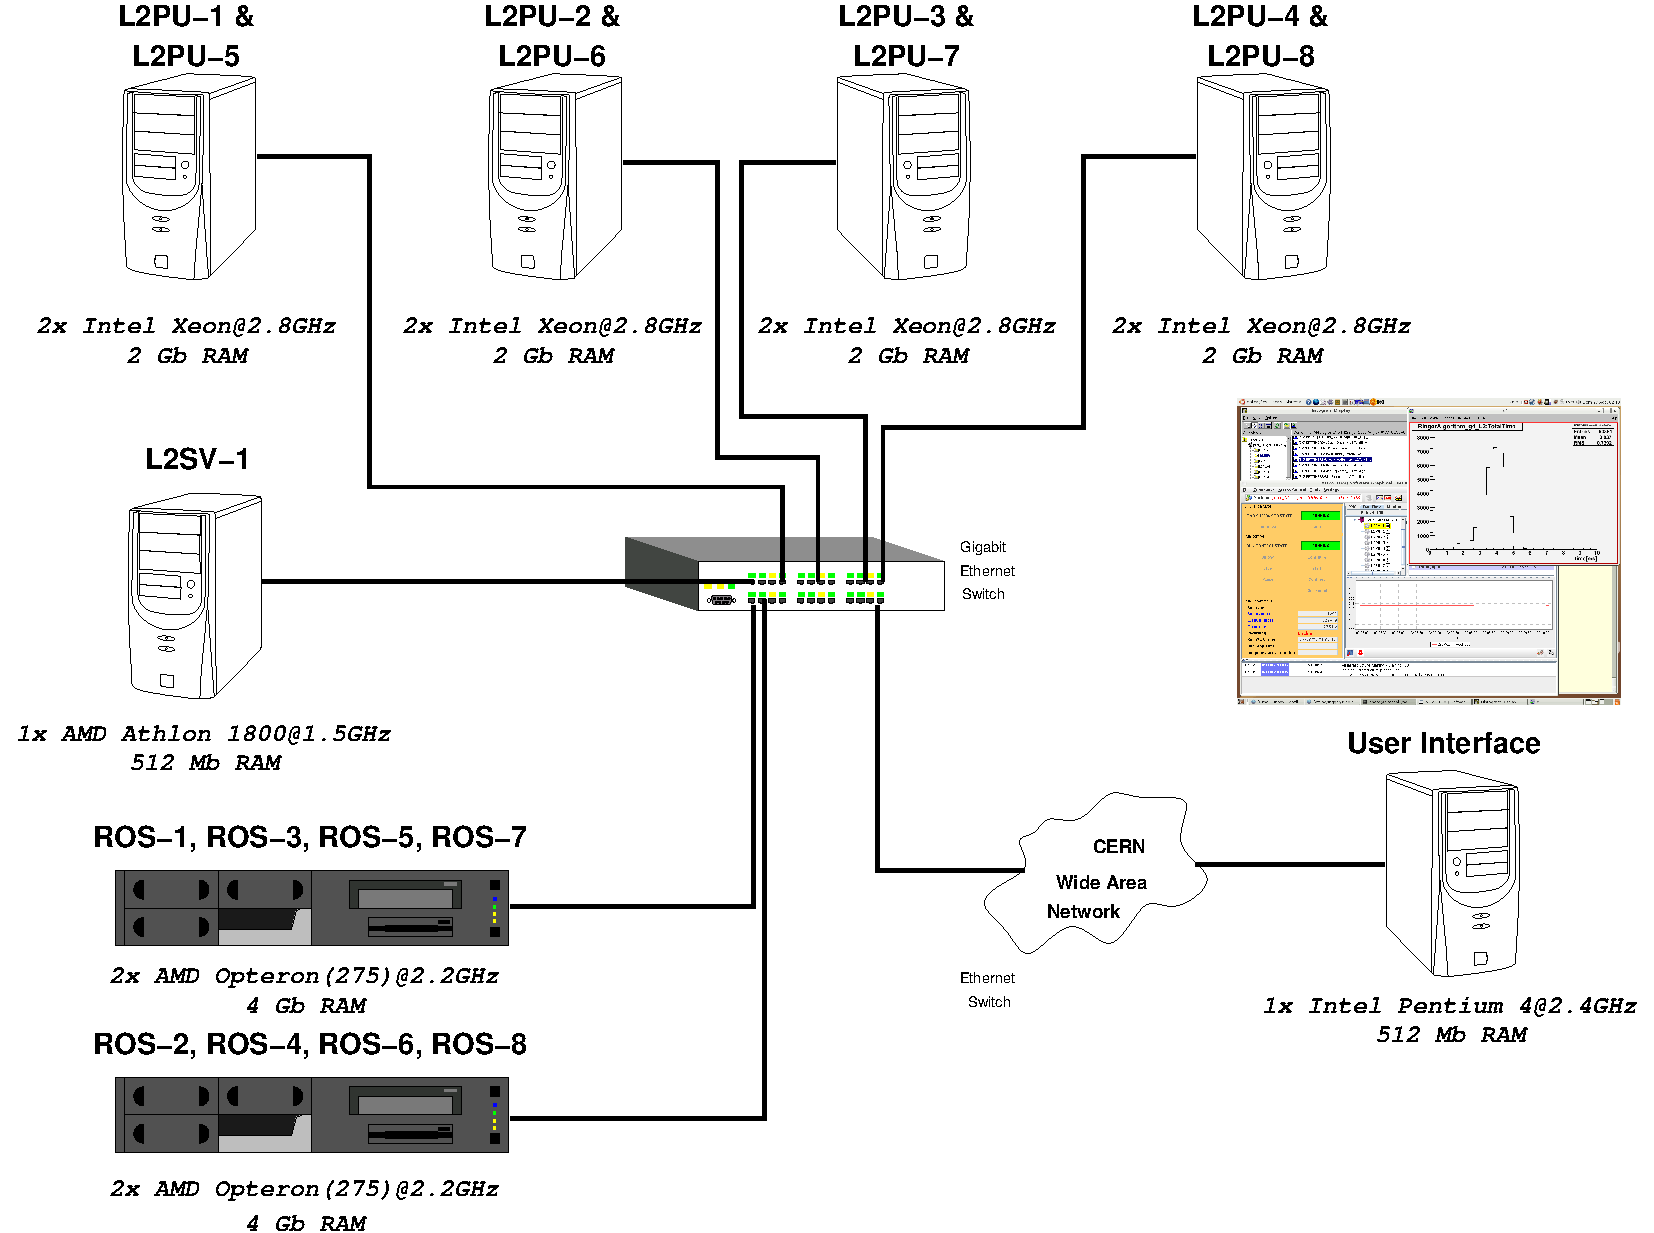
\includegraphics[scale=0.5]{online-schema}
\end{center}
\caption{Esquema de bancada de testes para a verificação do funcionamento do
NeuralRinger dentro do ambiente de aquisição de dados do ATLAS.}
\label{fig:online-schema}
\end{figure}

O sistema de filtragem e aquisição do ATLAS provê um conjunto de ferramentas
que podem ser utilizadas para monitorar a execução do sistema. A
Figura~\ref{fig:ringer-screenshot} mostra uma captura de tela na máquina
controladora, mostrando algumas destas ferramentas em atuação durante o
teste. A luz verde na maior das janelas indica que o sistema está operante e
nenhum erro foi detetado. O número de eventos processado, no total, pelas oito
unidades de processamento é de aproximadamente meio milhão. O valor está
marcado em vermelho na parte inferior esquerda da figura. A taxa de
funcionamento do sistema parece estável em cerca de 245~Hz, como indica o
gráfico na parte inferior direita da figura. Na parte superior direita, uma
janela do sistema de monitoração \eng{online} mostra um histograma, preenchido
durante a execução do sistema e atualizado durante a operação com o tempo de
processamento de um dos algoritmos de anelamento rodando na L2PU número 2. O
tempo de processamento médio deste algoritmo nesta L2PU é de cerca de
3,8~ms. Este tempo inclui o tempo de acesso aos dados através da rede
\eng{Gigabit ethernet} levando-se em conta a configuração da bancada.

\begin{figure}
\begin{center}
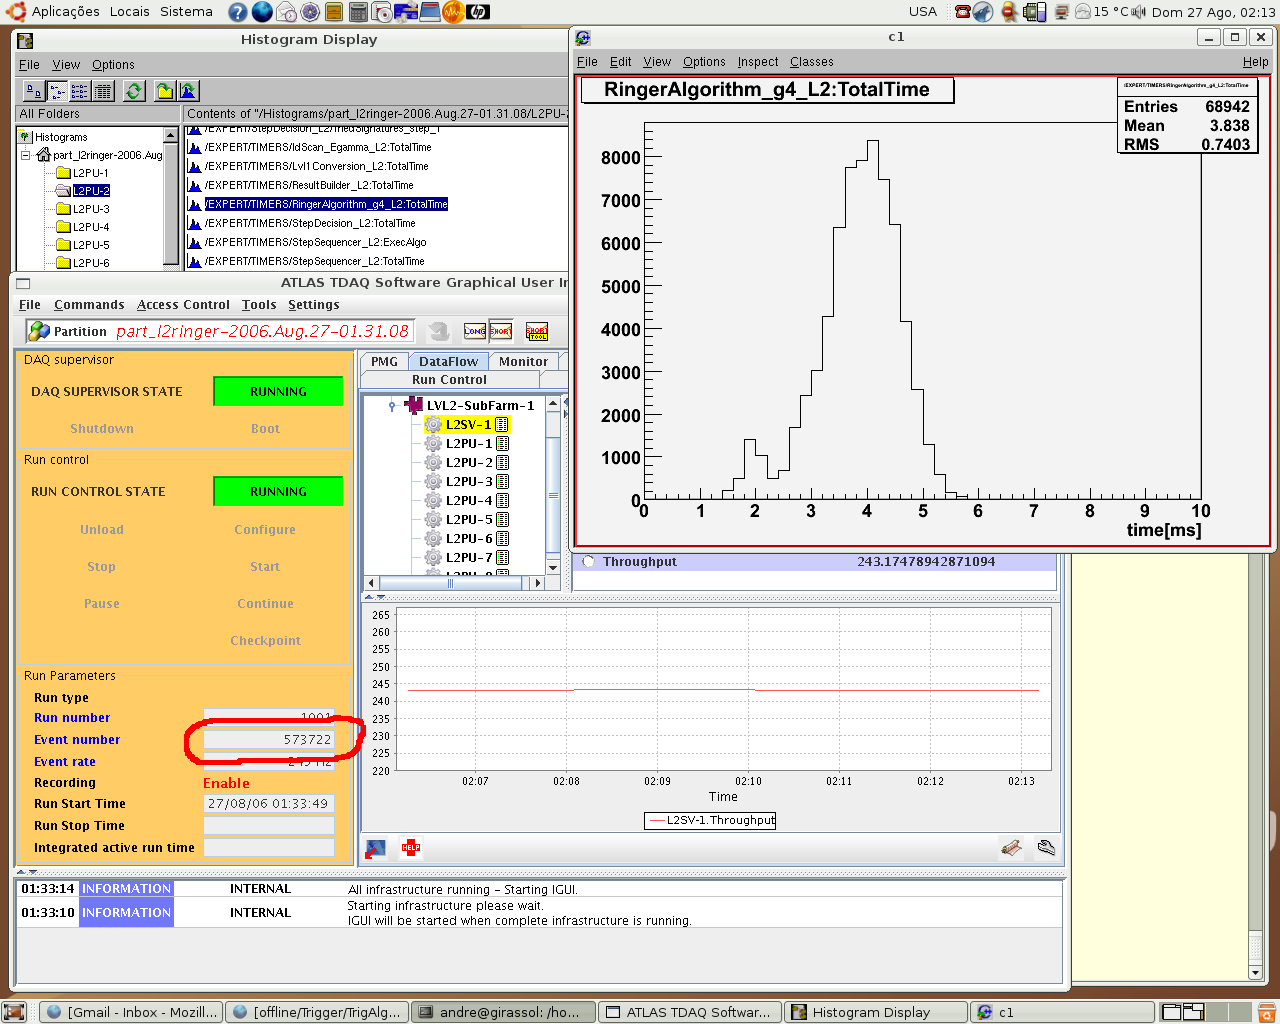
\includegraphics[scale=0.33]{ringer-online-3}
\end{center}
\caption{Captura de tela mostrando a operação do sistema de extração de
características baseado em anéis rodando dentro de uma banca de testes do
sistema de filtragem e aquisição do ATLAS.}
\label{fig:ringer-screenshot}
\end{figure}

\section{Implementação em um DSP}

As bibliotecas de anelamento e processamento neural, desenvolvidas no contexto
do \eng{NeuralRinger} (veja Apêndice~\ref{ap:framework}), são extremamente
portáteis e podem ser utilizadas em plataformas domésticas ou
especialistas. Nesta seção, descrevemos uma implementação do
\eng{NeuralRinger}, baseada em DSP's (do inglês \eng{Digital Signal
Processors}), que pode ser utilizada como plataforma de desenvolvimento de
sistemas de anelamento e detetores neurais para operarem no Sistema de
Filtragem do ATLAS.

DSP's são dispositivos que implementam, de forma bastante eficaz, operações
vetoriais como somas e multiplicações seguidas de acumulação, \eng{buffers}
circulares sendo bastante eficientes em processos iterativos, como restrições
de operação em tempo-real \cite{dsp-first}. A Figura~\ref{fig:dsp-inner}
mostra algumas das diferenças fundamentais entre processadores de uso genérico
(abordados até aqui) e DSP's. Enquanto processadores genéricos possuem apenas
uma unidade lógica aritmética, com apenas um barramento para transportar
instruções e dados \cite{rt-signal-proc}, DSP's contêm, adicionalmente, um
sistema de multiplicação implementado em \eng{hardware}, conectado diretamente
à memória interna através de múltiplos barramentos. Ademais, DSP's são
normalmente dotados de dispositivos para entrada e saída dedicados,
adicionados para se obter acesso eficiente aos dados e de forma a manter as
unidades computacionais focadas somente no processamento lógico e aritmético.
Em específico para este estudo, o DSP utilizado foi um SHARC ADSP-21160 da
\eng{Analog Devices}, operando em ponto-flutuante, com 100 MHz de \eng{clock},
4 Mbits de memória interna e unidades aritméticas duplicadas para operação em
modo SIMD (do inglês \eng{Single-Instruction, Multiple Data})
\cite{adsp-21160-manual}. 

\begin{figure}
\begin{center}
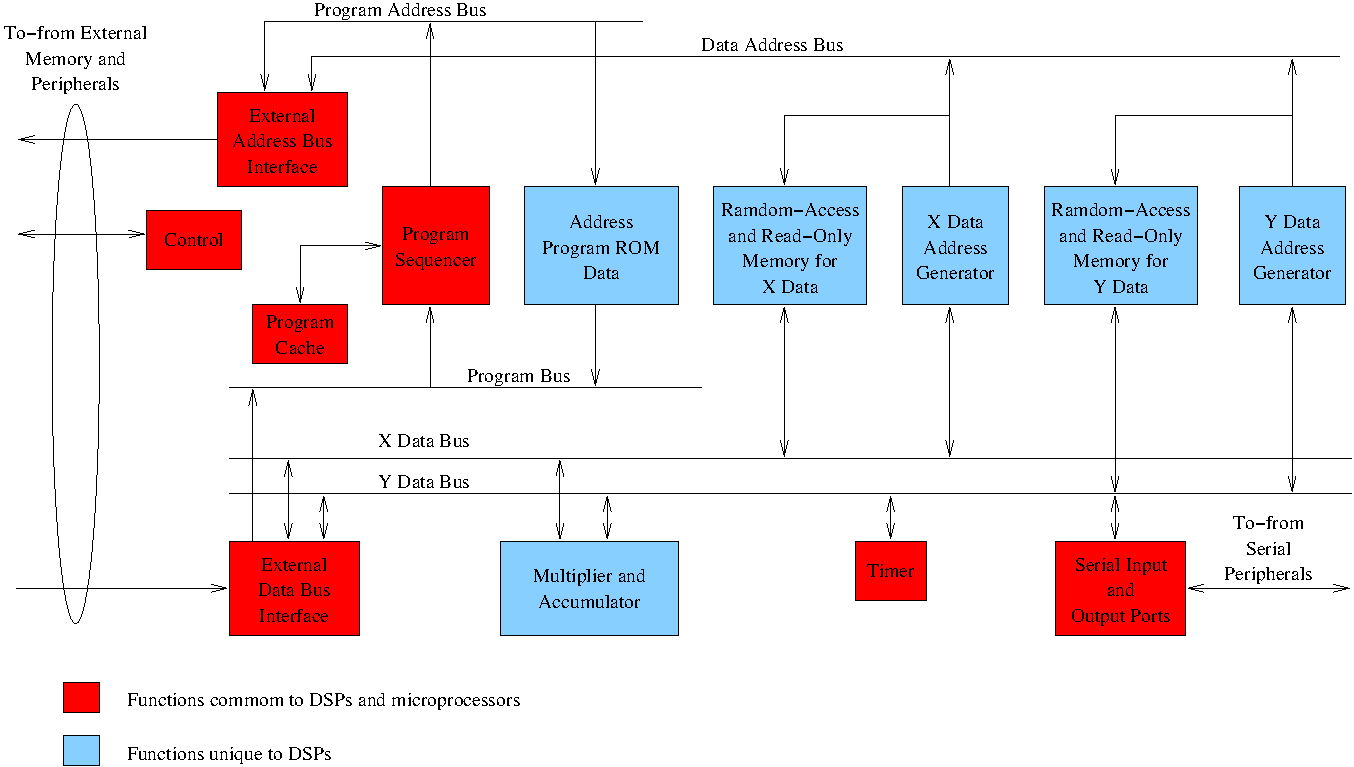
\includegraphics[width=\textwidth]{general_dsp_block_diagram}
\end{center}
\caption{Visão geral da estrutura interna de um DSP.}
\label{fig:dsp-inner}
\end{figure}

Desta forma, a parte central de computação do anelamento e deteção neural do
\eng{NeuralRinger} foi extraída, formando uma sub-estrutura de código 
diretamente focada no Sistema de Filtragem. Este código foi, sem maiores
modificações, re-compilado utilizando-se as ferramentas providas pelo
fabricante do DSP e operado dentro desta plataforma. 

Para a separação elétron/jato baseada em 100 anéis de deposição energética,
esta plataforma atinge um tempo de processamento de $4,692 \pm 1,108$
milissegundos por evento, que é compatível com os tempos de processamento
obtidos para execução dentro da pilha de \eng{software} do experimento, em
máquinas hipoteticamente 30 vezes mais rápidas. A Figura~\ref{fig:dsp-cumul}
mostra o tempo cumulativo (integral do histograma de distribuição dos tempos
de processamento) para este sistema, dividido em sub-fases do processamento. É
possível notar que a geração dos anéis seja, computacionalmente, a fase mais
importante do processamento, consumindo mais de 90\% do tempo total. Isto se
deve ao grande número de condições que rege a geração de anéis, nos afastando
do propósito operacional desta plataforma: multiplicações e acumulações
vetoriais, precedidas do pré-carregamento em, normalmente grandes
\eng{pipelines}. A fase de determinação do pico de deposição energética é a
segunda fase que mais consome tempo de processamento, por motivos idênticos
àqueles do anelamento. A normalização, juntamente com a deteção por métodos
neurais são as partes mais rápidas. A rede neural leva apenas, em média,
$10,43\pm0,47$ microssegundos por evento processado.


\begin{figure}
\begin{center}
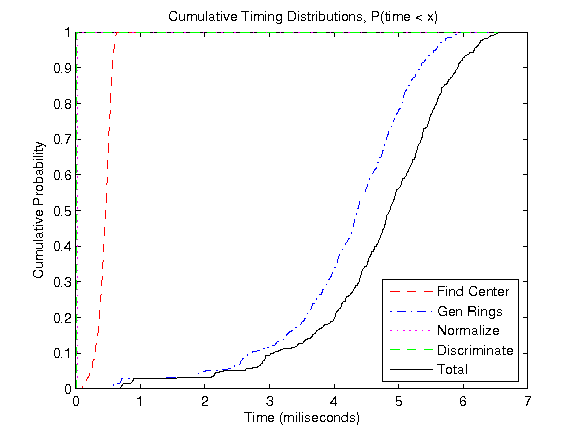
\includegraphics[width=\textwidth]{dsp_cumulative_time_distribution}
\caption{Função de distribuição cumulativa para os tempos de processamento,
subdivididos por fase de processamento, para implementação do
\eng{NeuralRinger} em um DSP SHARC 21160 da \eng{Analog Devices}.}
\label{fig:dsp-cumul}
\end{center}
\end{figure}

O tempo total de processamento encontrado neste exercício pode ser reduzido
considerando-se DSP's que operem com \eng{clocks} de freqüências mais altas. A
Figura~\ref{fig:dsp-clock-time} mostra os tempos totais de processamento que
poderiam ser atingidos com DSP's mais velozes da mesma família do sistema
atualmente empregado (SHARC). O tempo de execução nesta figura é obtido,
simplesmente, dividindo-se o número de instruções executadas no algoritmo (uma
vez que DSP's desta família executam instruções em apenas um ciclo do
\eng{clock}) pela freqüência do novo DSP. Como é possível ver, com um DSP de
400~MHz, o tempo total de processamento seria de apenas cerca de 1~ms.

\begin{figure}
\begin{center}
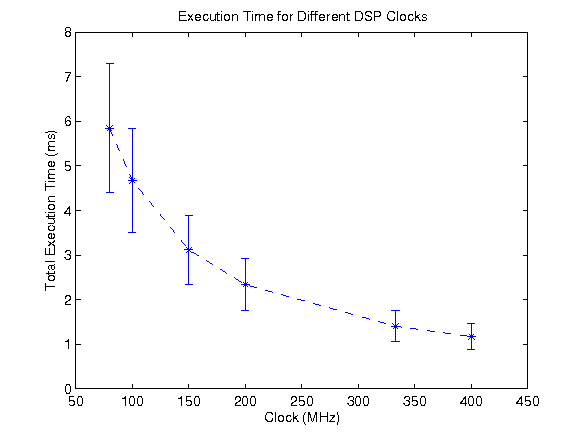
\includegraphics[width=\textwidth]{clock_scaling}
\caption{Tempo total de execução para o anelador e detetor neural para
diferentes DSP's da família SHARC, da \eng{Analog Devices}.}
\label{fig:dsp-clock-time}
\end{center}
\end{figure}

\typeout{ *************** End of file implement.tex *************** }
